In this subsection we provide some mockups that show an example of some possible user interface, one for the mobile app which will be available to the users and one for the web app available to the businesses, that offer the charging service.

\paragraph{EVD interaction with the mobile app of the eMall}
The EVD needs to download the mobile app on his cellphone in order to interact with the eMall and take advantage of its functionalities. The Graphical User Interface (GUI) of the application is thought as an user-friendly interface, to facilitate everyone in using the service. In this first mockup we see the initial page of the system, shown to the user when opening the application.
\begin{figure}[H]
    \centering
    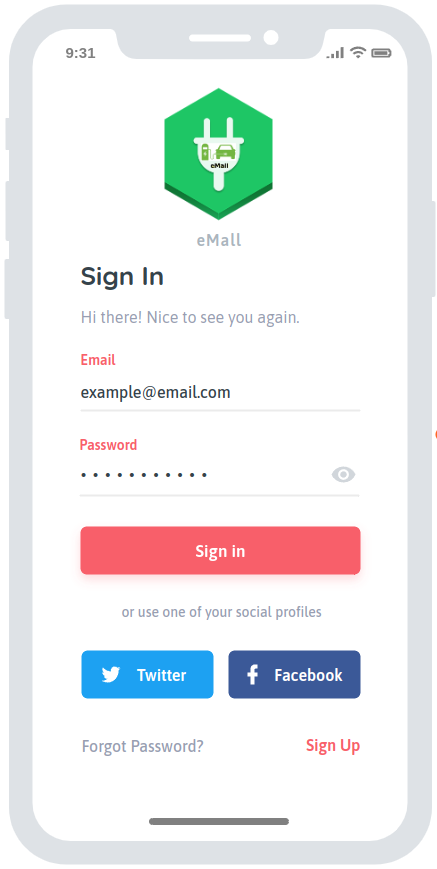
\includegraphics[scale=.3]{Images/cp3/signIn.png}
    \caption{Wireframe of the page that allows to log in from the eMma}
\end{figure}

In the following mockups we represent an example of the signing up procedure, showing the data required by the eMma in order to complete the creation of an account. 
\begin{figure}[H]
    \centering
    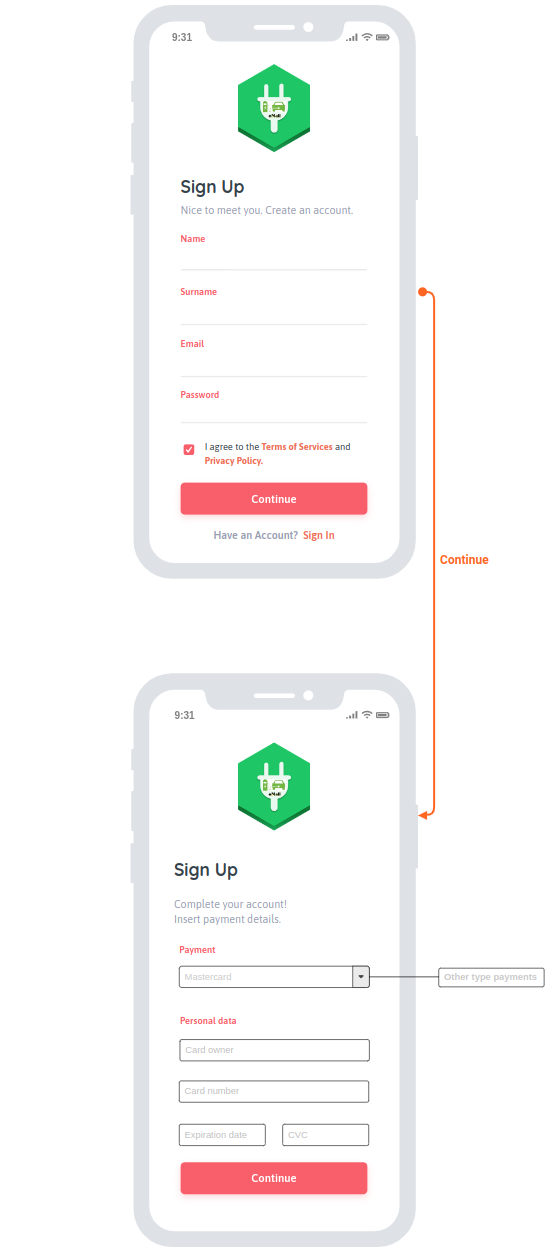
\includegraphics[scale=.45]{Images/cp3/signUp.png}
    \caption{Wireframe of the signing up process that allows to register from the eMma}
\end{figure}

\paragraph{CPO interaction with the managerial web app of the eMall}

